\chapter{Example chapter}
This is an example chapter with an example citation~\cite{tikhonov1977solutions}.


\section{Example section}
This is an example section.

% This is an example equation using some predefined formulas
\begin{equation}
    \resrad = \Tr(\matr{A})
\end{equation}

% These are example plots:
\begin{figure}[htp]
    \begin{subfigure}[b]{.38\textwidth}
        \centering
        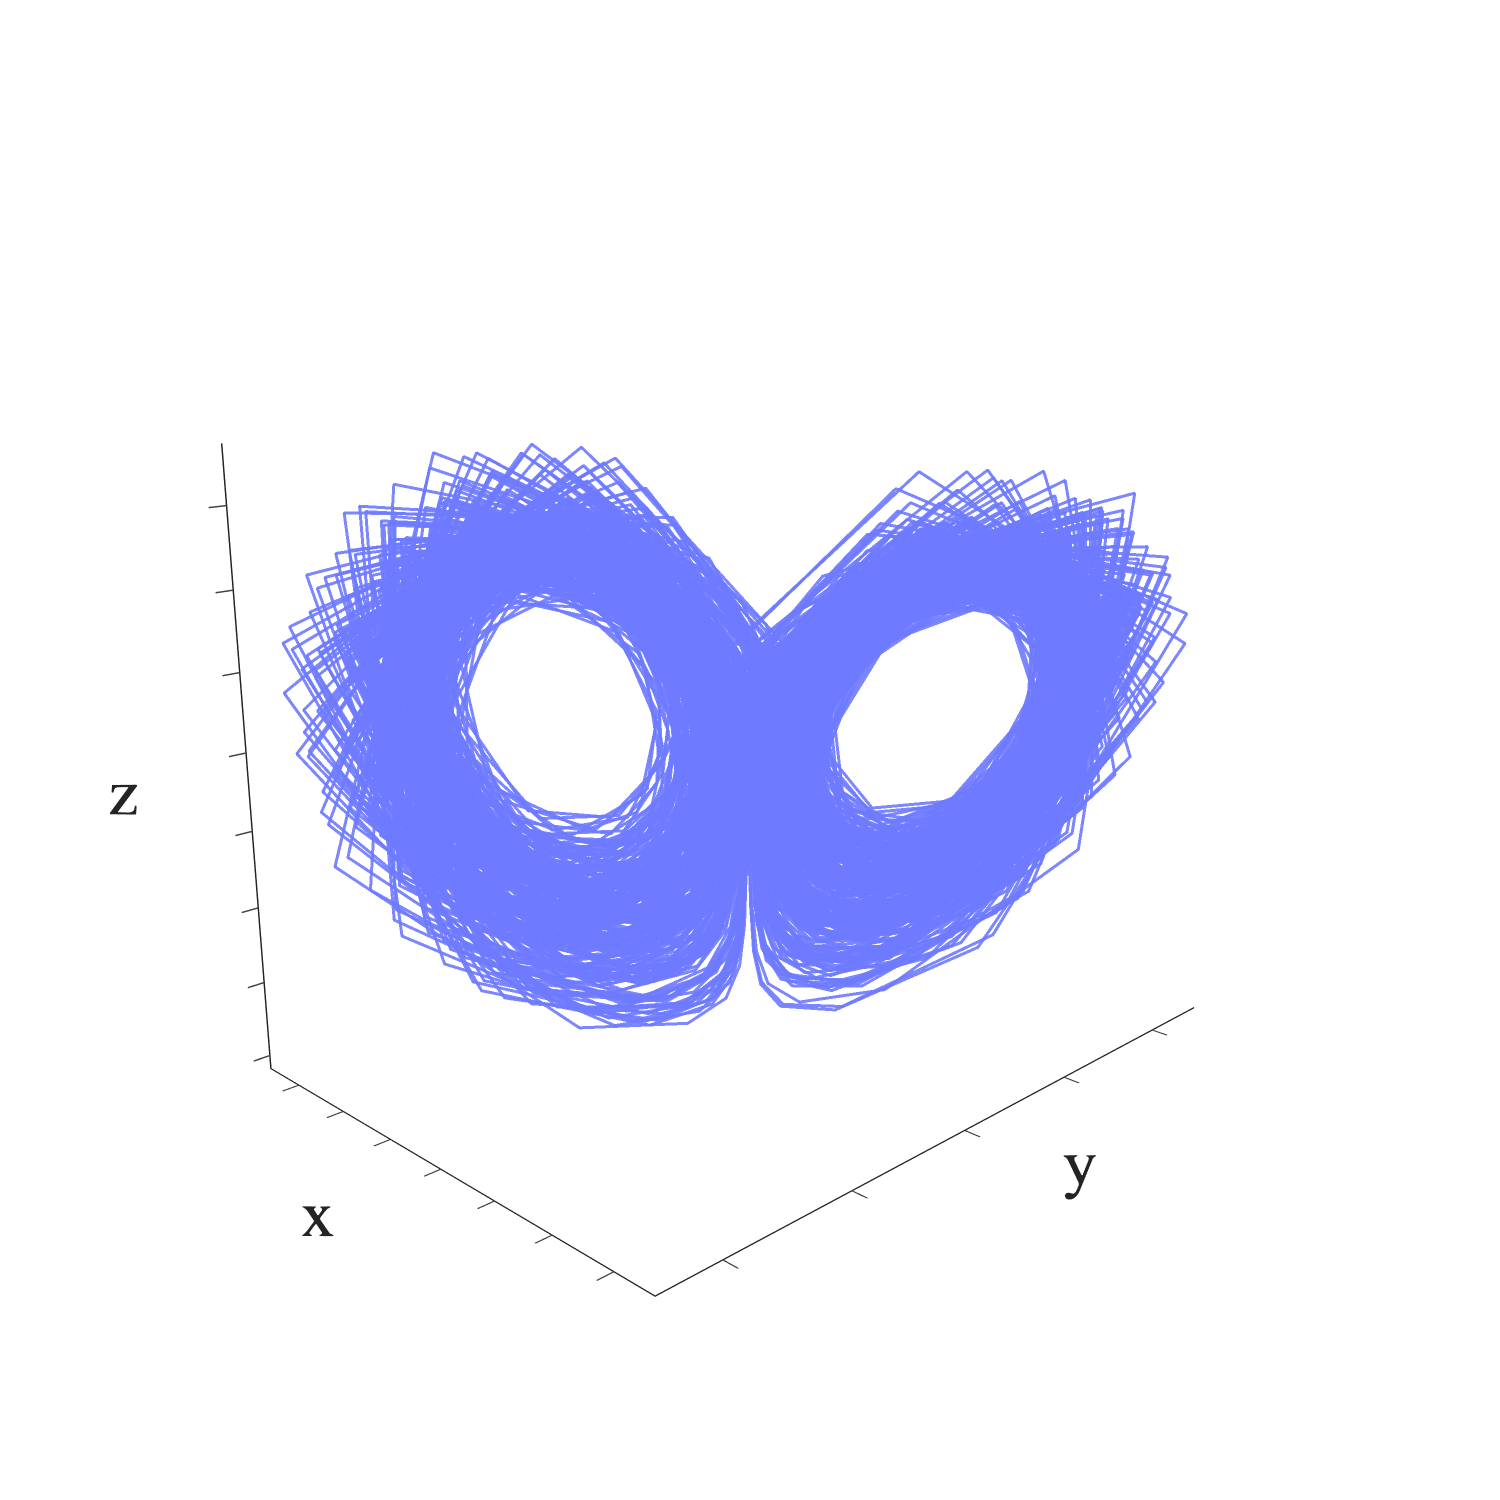
\includegraphics[width=.99\linewidth]{./figures/02_ExampleChapter/perturbed_vs_true_lorenz_traj}
        \caption{Lorenz attractor}
        \label{fig:lorenz-trajectory-basis-vs-pert}
    \end{subfigure}
    \begin{subfigure}[b]{.61\textwidth}
        \centering
        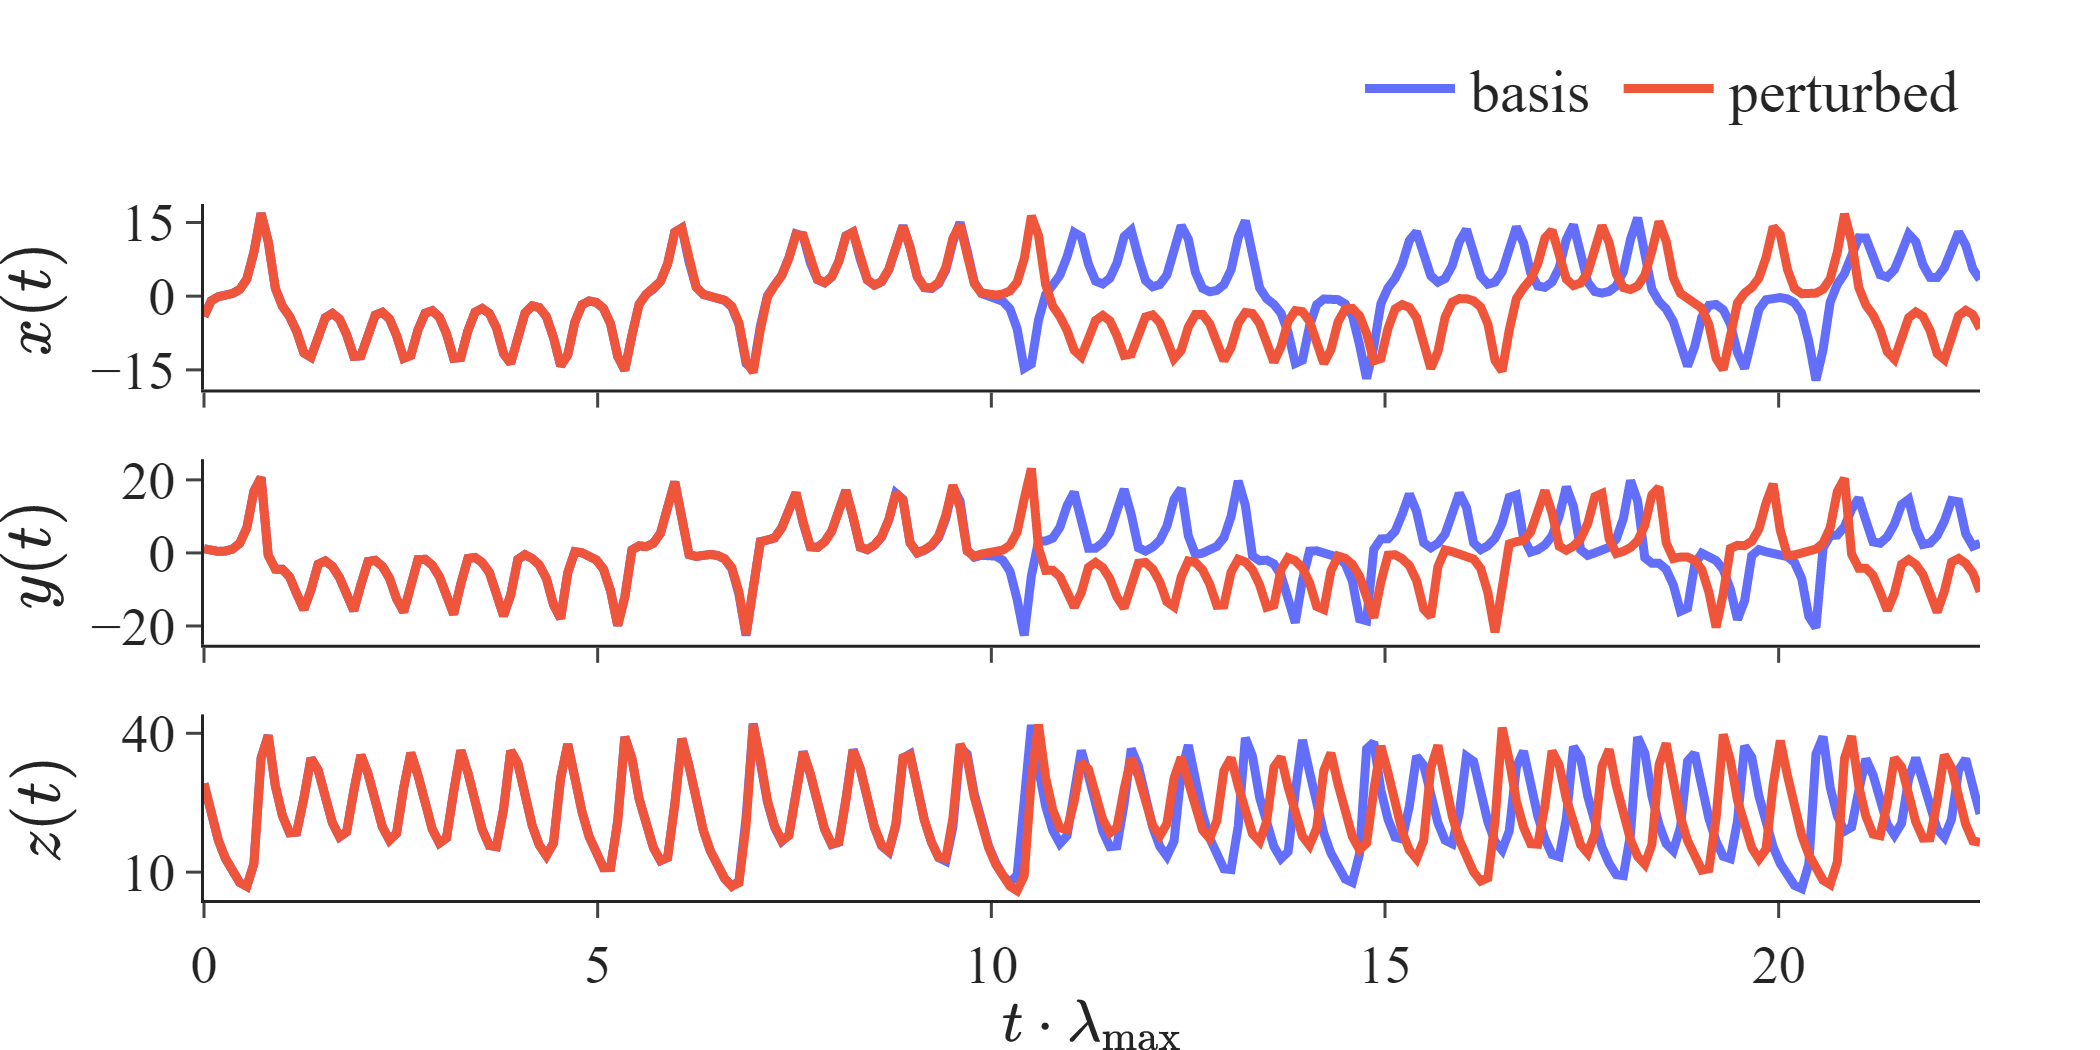
\includegraphics[width=.99\linewidth]{./figures/02_ExampleChapter/perturbed_vs_true_lorenz_1dim_all}
        \caption{Time series of initially nearby states}
        \label{fig:lorenz-timeseries-basis-vs-pert}
    \end{subfigure}
    \caption{
        Evolution of the Lorenz system.
    }
    \label{fig:lorenz-basis-vs-pert}
\end{figure}
